\section{Background information} % FIXME: improve name
\begin{frame}[t]{Explanations}{Jayvee}
	Jayvee is a language aiming to allow everyone to describe data pipelines \footcite{jvalue:jayvee}.
	\begin{figure}[h]
		\begin{center}
			\includesvg[width=0.5\linewidth]{assets/etl.svg}
		\end{center}
		\caption{The basic structure of a pipeline \footcite{jvalue:jayvee:docs:core_concepts}}
	\end{figure}
	\pause
	Examples:
	\begin{description}
		\item[Extractor] \Verb|HttpExtractor|, \Verb|LocalFileExtractor|
		\item[Transformer] \Verb|CSVInterpreter|, \Verb|TableTransforemer|
		\item[Loader] \Verb|CSVFileLoader|, \Verb|SQLiteLoader|
	\end{description}
\end{frame}


\begin{frame}[t]{Explanations}{Columnar storage}
	\begin{columns}[t]
		\begin{column}[t]{0.4\linewidth}
			\begin{itemize}
				\item Values are saved column after column\footnotemark.
				\item<2-> Advantages over row-oriented storage:
				      \begin{itemize}
					      \item Column specific compression\footnotemark
					      \item Less memory usage\footnotemark[2]
					      \item Faster read times\footnotemark[1]
				      \end{itemize}

			\end{itemize}
		\end{column}
		\hfill
		\begin{column}{0.6\linewidth}
			\begin{figure}
				\centering
				\begin{subfigure}{0.8\linewidth}
					\centering
					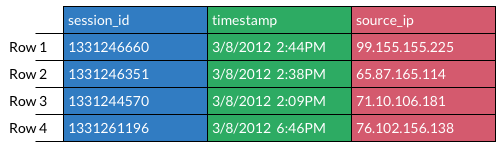
\includegraphics[height=0.2\FrameHeight]{assets/table-example}
					\caption{An example table in \dots}
				\end{subfigure}
				\\
				\begin{subfigure}{0.4\linewidth}
					\centering
					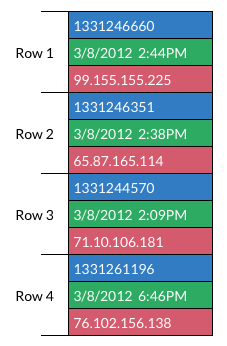
\includegraphics[height=0.3\FrameHeight]{assets/table-row}
					\caption{\dots row-oriented memory.}
				\end{subfigure}
				\begin{subfigure}{0.4\linewidth}
					\centering
					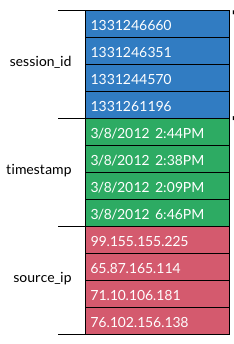
\includegraphics[height=0.3\FrameHeight]{assets/table-columnar}
					\caption{\dots columnar memory.}
				\end{subfigure}
				\caption{A table's is representation in row-oriented and columnar memory\footnotemark[3].}
			\end{figure}
		\end{column}
	\end{columns}
	\footnotetext[1]{\textcite{Floratou2019}}
	\footnotetext[2]{\textcite{Abadi2013}}
	\footnotetext[3]{\textcite{arrow:overview}}
\end{frame}

\begin{frame}[t]{Explanations}{Apache Arrow}
	\begin{columns}[t]
		\begin{column}{0.4\linewidth}
			Apache Arrow specifies:
			\begin{itemize}
				\item A memory format\footnotemark \text{ }that is:
				      \begin{itemize}
					      \item Columnar
					      \item In-memory
					      \item Language agnostic
				      \end{itemize}
				\item<3-> An IPC file format\footnotemark
			\end{itemize}
		\end{column}
		\hfill
		\begin{column}{0.6\linewidth}
			\centering
			\only<2> {
				\begin{figure}
					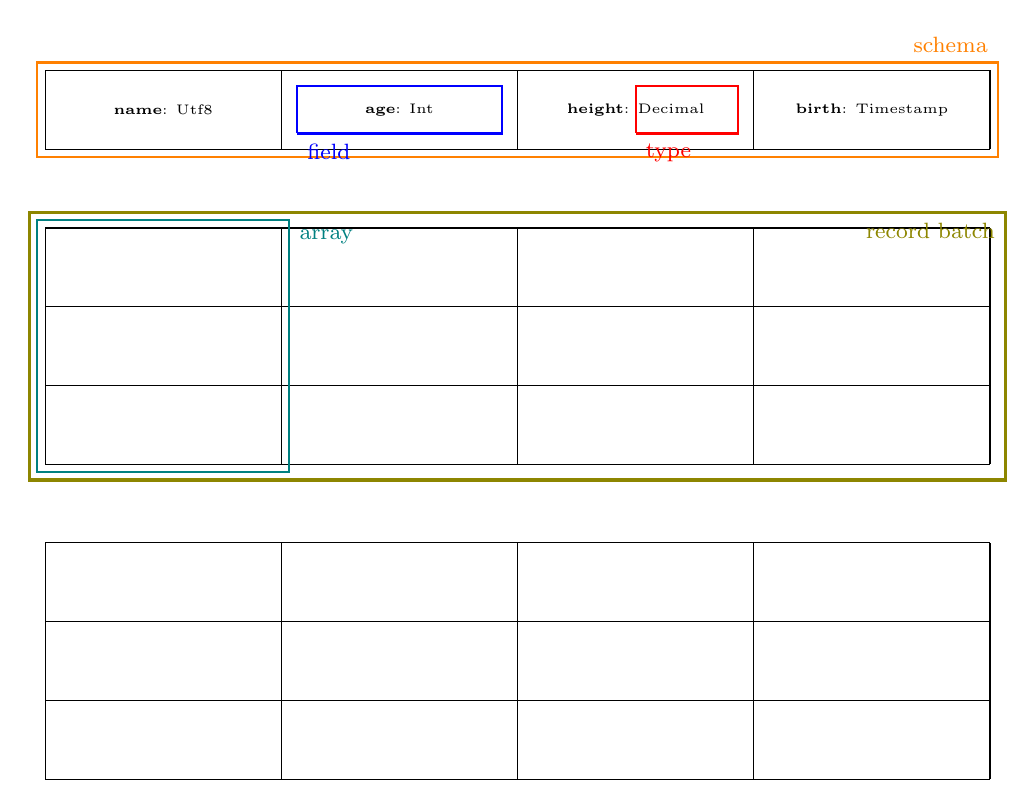
\begin{tikzpicture}
						\draw (0,0) -- (12,0)
						(0,1) -- (12,1)
						(0,2) -- (12,2)
						(0,3) -- (12,3)
						(0,4) -- (12,4)
						(0,5) -- (12,5)
						(0,6) -- (12,6)
						(0,7) -- (12,7)
						(0,8) -- (12,8)
						(0,9) -- (12,9)
						(0,0) -- (0,3) (0,4) -- (0,7) (0,8) -- (0,9)
						(3,0) -- (3,3) (3,4) -- (3,7) (3,8) -- (3,9)
						(6,0) -- (6,3) (6,4) -- (6,7) (6,8) -- (6,9)
						(9,0) -- (9,3) (9,4) -- (9,7) (9,8) -- (9,9)
						(12,0) -- (12,3) (12,4) -- (12,7) (12,8) -- (12,9);
						\node[] at (1.5,8.5) {\tiny \textbf{name}: Utf8};
						\node[] at (4.5,8.5) {\tiny \textbf{age}: Int};
						\node[] at (7.5,8.5) {\tiny \textbf{height}: Decimal};
						\node[] at (10.5,8.5) {\tiny \textbf{birth}: Timestamp};
						\draw[orange,thick] (-0.1,7.9) rectangle (12.1,9.1) node[anchor=south east]{\footnotesize schema};
						\draw[blue,thick] (3.2,8.2) -- (5.8,8.2) -- (5.8,8.8) -- (3.2,8.8) -- (3.2,8.2) node[anchor=north west] {\footnotesize field};
						\draw[red,thick] (7.5,8.2) -- (8.8,8.2) -- (8.8,8.8) -- (7.5,8.8) -- (7.5,8.2) node[anchor=north west] {\footnotesize type};
						\draw[teal,thick] (-0.1,3.9) rectangle (3.1,7.1) node[anchor=north west]{\footnotesize array};
						\draw[olive, very thick] (-0.2,3.8) rectangle (12.2,7.2) node[anchor=north east]{\footnotesize record batch};

					\end{tikzpicture}
					\caption{Key concepts of an Arrow table\footnotemark}
				\end{figure}
			}
			\only<3>{
				\begin{figure}
					\centering
					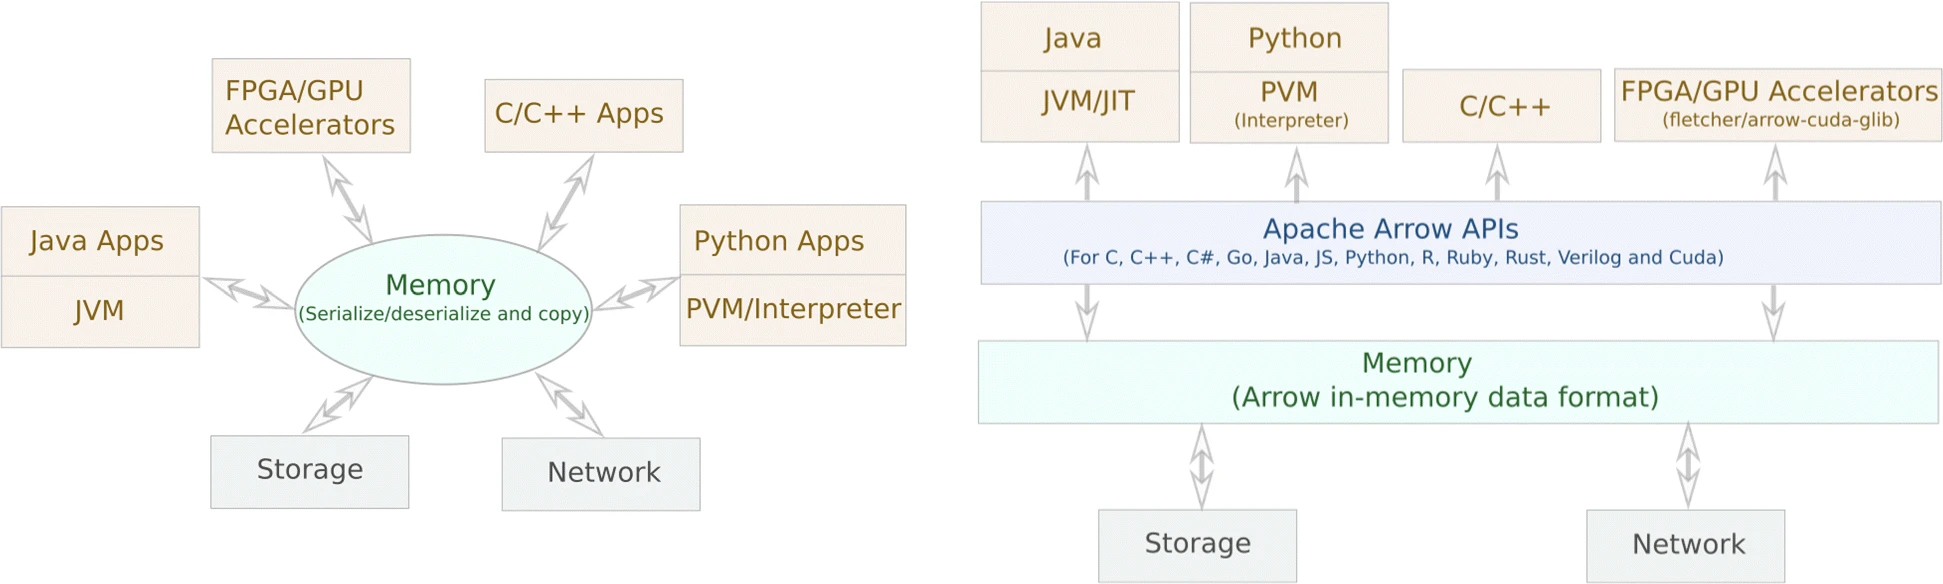
\includegraphics[width=0.9\linewidth]{assets/arrow_interop.png}
					\caption{Illustration demonstrating Arrow enhances interoperability between
						processes} % FIXME caption
				\end{figure}
			}
		\end{column}
		\hfill
	\end{columns}
	\footnotetext[1]{\textcite{arrow:spec}}
	\footnotetext[2]{\textcite{arrow:spec:ipc}}
	\footnotetext[3]{\textcite{Dremio}}
\end{frame}
\begin{frame}[t]{Explanations}{Polars}
	\begin{itemize}
		\item Polars is built on top of Apache Arrow\footnotemark[1]
		\item Provides additional abstractions, such as \Verb|DataFrame| and \Verb|Series|\footnotemark[1]
		\item Promises "up to 50x performance"\footnotemark[1]
	\end{itemize}
	\footnotetext[1]{\textcite{polars}}
\end{frame}


